% concatenated from causal_description_gap.tex
\documentclass{article}

% Pass natbib options BEFORE loading neurips_2026
\PassOptionsToPackage{numbers,sort&compress}{natbib}

% NeurIPS 2026 style with [preprint] option:
%   - de-anonymizes the author block,
%   - removes line numbers,
%   - adds "Preprint. Work in progress." footer.
% This is the recommended mode for arXiv distribution per the style file.
\usepackage[preprint]{neurips_2026}

% Encoding / fonts
\usepackage[utf8]{inputenc}
\usepackage[T1]{fontenc}
\usepackage{microtype}
\usepackage{xcolor}

% Math
\usepackage{amsmath,amsthm,amssymb,amsfonts}
\usepackage{mathtools}
\usepackage{thmtools}

% Graphics and figures
\usepackage{graphicx}
\usepackage{tikz}
\usetikzlibrary{arrows.meta,positioning,shapes,calc,decorations.pathreplacing}

% Tables
\usepackage{booktabs}
\usepackage{array}

% Plots
\usepackage{pgfplots}
\pgfplotsset{compat=1.17}

% Hyperlinks
\usepackage{url}
\usepackage[hidelinks]{hyperref}

% Theorem environments
\theoremstyle{plain}
\newtheorem{theorem}{Theorem}[section]
\newtheorem{lemma}[theorem]{Lemma}
\newtheorem{proposition}[theorem]{Proposition}
\newtheorem{corollary}[theorem]{Corollary}

\theoremstyle{definition}
\newtheorem{definition}[theorem]{Definition}
\newtheorem{example}[theorem]{Example}
\newtheorem{remark}[theorem]{Remark}

% Custom commands
\newcommand{\R}{\mathbb{R}}
\newcommand{\N}{\mathbb{N}}
\newcommand{\E}{\mathbb{E}}
\newcommand{\Prob}{\mathbb{P}}
\newcommand{\calM}{\mathcal{M}}
\newcommand{\calF}{\mathcal{F}}
\newcommand{\calA}{\mathcal{A}}
\newcommand{\Obs}{\mathsf{Obs}}
\newcommand{\Int}{\mathsf{Int}}
\newcommand{\CF}{\mathsf{CF}}
\newcommand{\DL}{\mathrm{DL}}
\newcommand{\pa}{\mathrm{pa}}
\newcommand{\Desc}{\mathrm{Desc}}
\DeclareMathOperator{\doop}{do}
\newcommand{\Ans}{\mathrm{Ans}}

\title{The Causal Description Gap:\\
Information-Theoretic Separations Across Pearl's Hierarchy}

\author{%
  Seyed Morteza Emadi \\
  Kenan-Flagler Business School \\
  University of North Carolina at Chapel Hill \\
  \texttt{seyed\_emadi@kenan-flagler.unc.edu}%
}

\begin{document}

\maketitle

\begin{abstract}
Pearl's causal hierarchy shows that observational, interventional, and counterfactual queries are qualitatively distinct. We ask a quantitative version of this question: how many additional bits are needed to specify higher-rung causal answers once lower-rung answers are known? We formalize this via \emph{query-class description length}, the Kolmogorov complexity of the answer oracle induced by an SCM for a class of queries. Our main construction gives binary acyclic SCMs whose observational distribution has constant description length, while the single-variable interventional answer oracle has description length $\Theta(n^2)$. A degree-sensitive upper bound shows that finite-gate-schema SCMs of indegree $d$ have observational--interventional gap at most $O(nd\log(en/d)+n\log n)$, making the quadratic construction order-optimal in the dense regime and a rooted-tree construction order-optimal for bounded indegree. The quadratic separation persists under $\varepsilon$-accurate total-variation descriptions for every fixed $\varepsilon<1/4$. At the next rung, the full hard-do interventional oracle can still leave a $\Theta(n)$ counterfactual description gap. A general ambiguity-to-bits theorem and Shannon analogue show that these gaps equal the logarithm of residual higher-rung ambiguity up to lower-order terms.
\end{abstract}


%==============================================================================
%==============================================================================
\section{Introduction}
\label{sec:intro}
%==============================================================================

Predictive accuracy identifies what a system does under passive observation. \emph{Causal} questions go further: \emph{interventional} queries (``what if I set $X$?'') and \emph{counterfactual} queries (``what would have happened if $X$ had been different?''). Pearl's causal hierarchy~\citep{pearl2009causality} formalizes these three levels (association, intervention, counterfactual), and the Causal Hierarchy Theorem~\citep{bareinboim2022pearl} shows the hierarchy is generically strict: higher-rung queries cannot in general be answered from lower-rung information. But \emph{how large} is the gap? Is the additional information bounded by a constant, or can it scale with system size?

We give a quantitative answer in bits. For a structural causal model $M$, we define \emph{query-class description lengths} $\DL_1(M), \DL_2(M), \DL_3(M)$ as the Kolmogorov complexities (conditional on $n$) of the observational, interventional, and counterfactual answer objects, and \emph{causal description gaps} $\Delta_{2|1}, \Delta_{3|2}$ as the additional bits needed conditional on the lower rung. The framework lets us treat ``how much causal information is missing'' as a precise quantity.

\paragraph{Residual information after non-identification.}
Existing hierarchy and identifiability results ask whether a higher-rung answer is determined by lower-rung information. We study the \emph{residual-information problem} that remains when identification fails: among all SCMs that agree on the lower-rung answer, how many bits are still needed to specify the higher-rung answer oracle? Our separations refine non-identifiability from a Boolean obstruction into a quantitative information measure. The familiar two-variable ambiguity $X \to Y$ versus $X \leftarrow Y$ via deterministic copy is the one-bit version of this phenomenon; our main construction scales it to $2^{\Theta(n^2)}$ residual mechanisms, forcing a $\Theta(n^2)$-bit gap.

\paragraph{Contributions.}
\begin{enumerate}
    \item \textbf{Framework.} We turn Pearl's qualitative hierarchy into a quantitative information hierarchy by defining query-class description length and causal description gaps: the residual bits needed to specify higher-rung answer oracles after lower-rung answers are fixed (\S\ref{sec:framework}).
    \item \textbf{Observational--interventional separations and degree-sensitive optimality.} Explicit SCM families with constant observational description length but $\Theta(n \log n)$ and $\Theta(n^2)$ interventional gaps (\S\ref{sec:warmup}--\S\ref{sec:quadratic}); a matching upper bound $O(nd \log(en/d) + n \log n)$ for finite-gate-schema SCMs of indegree $d$, making the tree and bipartite constructions order-optimal at $d = O(1)$ and $d = \Theta(n)$ (\S\ref{sec:degree-optimality}).
    \item \textbf{Finite-precision and learning consequences.} The quadratic gap survives $\varepsilon$-accurate total-variation descriptions for every $\varepsilon < 1/4$ (\S\ref{sec:finite-precision}); consequently no observational learner beats the $2^{-m^2}$ guessing rate in our family (\S\ref{sec:learning-main}).
    \item \textbf{Counterfactual gap and unifying ambiguity principle.} Mechanisms with identical full hard-do oracles can still differ by $\Theta(n)$ counterfactual bits (\S\ref{sec:counterfactual}); a general ambiguity-to-bits theorem and Shannon analogue show these gaps equal the log of residual higher-rung ambiguity up to lower-order terms (\S\ref{sec:general}).
\end{enumerate}

\paragraph{Summary of constructions.}
Table~\ref{tab:summary} previews the three SCM families used to instantiate the framework. All three have constant-bit lower-rung descriptions; the gap in each row is at least the log of the higher-rung ambiguity (Theorem~\ref{thm:ambiguity-bits}), and is matched by an explicit upper-bound encoding.

\begin{table}[h]
\centering
\small
\begin{tabular}{@{}lccccl@{}}
\toprule
\textbf{Family} & \textbf{Lower rung} & \textbf{Higher rung} & \textbf{Ambiguity} & \textbf{Gap} & \textbf{Where} \\
\midrule
Rooted trees     & $\Obs$              & $\Int_1$            & $n^{n-1}$ & $\Theta(n \log n)$ & \S\ref{sec:warmup} \\
Bipartite graphs & $\Obs$              & $\Int_1$            & $2^{m^2}$ & $\Theta(n^2)$      & \S\ref{sec:quadratic} \\
Modular XOR      & $\Int_{\mathrm{all}}$ & $\CF_1$           & $2^m$     & $\Theta(n)$        & \S\ref{sec:counterfactual} \\
\bottomrule
\end{tabular}
\caption{Three SCM families instantiating the framework. ``Lower / Higher rung'' name the query classes between which the gap is measured; ``Ambiguity'' is the number of higher-rung answer objects consistent with a single lower-rung answer.}
\label{tab:summary}
\end{table}

\section{Related Work}
\label{sec:related}
%==============================================================================

\paragraph{Pearl's causal hierarchy.}
Pearl's three-level hierarchy~\citep{pearl2009causality,pearl2018book} is generically strict: the Causal Hierarchy Theorem~\citep{bareinboim2022pearl} establishes non-identifiability, showing that some higher-rung queries are not functions of lower-rung information. \citet{shpitser2008complete} give complete identification algorithms; \citet{ibeling2023comparing} compare frameworks. We quantify the size of the residual answer set: even for simple binary acyclic SCMs, its description length can be $\Theta(n^2)$.

\paragraph{Causal discovery.}
Constraint- and score-based methods identify causal graphs up to Markov equivalence from observations~\citep{spirtes2000causation,peters2017elements,hauser2012characterization}. \citet{eberhardt2005number} and \citet{shanmugam2015learning} bound the number/sample complexity of interventions for identification. We give description-length lower bounds: even with infinite observational data, the obs--int information gap is $\Theta(n^2)$ in our family.

\paragraph{Description length and MDL.}
Kolmogorov complexity~\citep{kolmogorov1965three,li2008introduction} and MDL~\citep{grunwald2007minimum} measure the information needed to describe objects or models. Our use is different: the compressed object is neither the dataset nor the SCM parameterization, but the \emph{answer oracle} for a query class. This distinction is what enables our separations: the observational answer oracle can have constant description length even when the corresponding interventional oracle requires $\Theta(n^2)$ bits.

\paragraph{Causal reasoning in AI.}
Recent benchmarks find uneven causal-reasoning performance in LLMs~\citep{kiciman2023causal,jin2024cladder}; our results give one information-theoretic reason why observational predictive training alone need not induce interventional competence in worst-case structured families.

\paragraph{Complexity across Pearl's hierarchy.}
\citet{dorfler2024complexity} study satisfiability across probabilistic, interventional, and counterfactual languages in Pearl's hierarchy, proving strictly increasing computational complexity for certain languages (e.g., NP$^{\mathrm{PP}}$, PSPACE, and NEXP completeness under addition and marginalization). Their setting assumes the SCM is given and asks how hard it is to decide whether causal statements are jointly satisfiable; we bound the \emph{information content} of higher-rung answer oracles given lower-rung ones, providing complementary views on the cost of climbing the hierarchy.


%==============================================================================
\section{Framework: Query-Class Description Length}
\label{sec:framework}
%==============================================================================

\subsection{Structural Causal Models}
\label{sec:scm-review}

\begin{definition}[Structural Causal Model]
A \emph{structural causal model} (SCM) on binary variables $X_1, \ldots, X_n \in \{0,1\}$ is a tuple $M = (G, \{f_i\}, P_U)$ where:
\begin{itemize}
    \item $G$ is a directed acyclic graph (DAG) on $[n] := \{1, \ldots, n\}$.
    \item $U_1, \ldots, U_n$ are independent exogenous (noise) variables with distribution $P_U$.
    \item Structural equations specify each variable as a function of its parents and noise:
    \[
    X_i = f_i\bigl( (X_j)_{j \in \pa_G(i)}, U_i \bigr).
    \]
\end{itemize}
We require $f_i$ to be computable and $P_U$ to have rational probabilities, ensuring all quantities are well-defined.
\end{definition}

The SCM generates data as follows: sample $(U_1, \ldots, U_n) \sim P_U$, then compute $X_i$ in topological order. The resulting distribution $P_M(X_1, \ldots, X_n)$ is the \textbf{observational distribution}.

\begin{definition}[Intervention]
An \emph{intervention} $\doop(X_i = x)$ modifies $M$ by replacing the equation for $X_i$ with the constant $X_i := x$, leaving all other equations unchanged. The resulting distribution is $P_M^{\doop(X_i = x)}$.
\end{definition}

Interventions are the formal model of ``what happens if we force $X_i$ to take value $x$, breaking its dependence on its natural causes.''

\begin{definition}[Counterfactual]
For a fixed exogenous realization $u = (u_1, \ldots, u_n)$, the \emph{counterfactual} $X^{(i \leftarrow b)}(u)$ is the value of the entire system $(X_1, \ldots, X_n)$ when we intervene with $\doop(X_i = b)$ but use the \emph{same} noise realization $u$.

Counterfactual queries ask about joint distributions like $P(X, X^{(i \leftarrow 0)}, X^{(i \leftarrow 1)})$: the ``parallel worlds'' where we observe the actual outcome and both hypothetical interventions, all computed from the same underlying noise.
\end{definition}

\subsection{Query Families: What We Need to Specify}
\label{sec:query-families}

To measure information content at each level of the hierarchy, we define what must be specified to answer all queries at that level.

\begin{definition}[Query Families]
\label{def:query-families}
For an SCM $M$ on $n$ variables:
\begin{itemize}
    \item \textbf{Observational:} $\Obs(M) := P_M$, the joint distribution over $(X_1, \ldots, X_n)$.
    
    \item \textbf{Single-node interventional:}
    \[
    \Int_1(M) := \Bigl( P_M,\, \bigl(P_M^{\doop(X_i = 0)}, P_M^{\doop(X_i = 1)}\bigr)_{i=1}^n \Bigr).
    \]
    This lists the observational distribution plus the $2n$ single-variable interventional distributions.
    
    \item \textbf{Single-node counterfactual:}
    \[
    \CF_1(M) := \Bigl( P\bigl(X, X^{(i \leftarrow 0)}, X^{(i \leftarrow 1)}\bigr) \Bigr)_{i=1}^n.
    \]
    For each variable $i$, this is the joint distribution of the actual world $X$ and the two counterfactual worlds under $\doop(X_i = 0)$ and $\doop(X_i = 1)$, evaluated on the same exogenous noise.
\end{itemize}
\end{definition}



\subsection{Description Lengths and the Causal Gap}
\label{sec:description-lengths}


\begin{definition}[Kolmogorov Complexity]
Fix a universal prefix-free Turing machine. The \emph{Kolmogorov complexity} $K(z)$ of a string $z$ is the length of the shortest program that outputs $z$. The conditional complexity $K(z \mid w)$ is the shortest program length when $w$ is given as auxiliary input. All equalities hold up to an additive $O(1)$ constant.
\end{definition}

Distributions are encoded as the string of their (rational, lowest-terms) probabilities; the choice of computable encoding affects $K$ only by $O(1)$.

\begin{definition}[Query-Class Description Length: General Form]
\label{def:qcdl-general}
Let $Q$ be a query class with a computable answer encoding $\Ans_Q(M)$ (a finite string summarizing the answers to all queries in $Q$ when posed to SCM $M$). The \emph{query-class description length} of $M$ with respect to $Q$ is
\[
\DL(Q;\, M) \;:=\; K\!\bigl(\Ans_Q(M) \mid n\bigr).
\]
The \emph{conditional gap} between query classes $Q_2$ and $Q_1$ is
\[
\Delta(Q_2 \mid Q_1;\, M) \;:=\; K\!\bigl(\Ans_{Q_2}(M) \mid \Ans_{Q_1}(M),\, n\bigr).
\]
\end{definition}


Specializing to the three rungs of the causal hierarchy gives the canonical lengths
$\DL_1(M) := K(\Obs(M) \mid n)$,
$\DL_2(M) := K(\Int_1(M) \mid n)$, and
$\DL_3(M) := K(\CF_1(M) \mid n)$.

\begin{lemma}[Counting bound for Kolmogorov complexity]
\label{lem:counting}
Let $z_1, \ldots, z_N$ be $N$ distinct strings and let $w$ be an arbitrary auxiliary string. Then:
\begin{enumerate}
    \item At least one $z_i$ satisfies $K(z_i \mid w) \geq \log_2 N - O(1)$.
    \item For every $c \geq 0$, all but at most a $2^{-c}$ fraction of the $z_i$ satisfy $K(z_i \mid w) \geq \log_2 N - c - O(1)$.
\end{enumerate}
The unconditional version ($w$ empty) is the special case. We apply this lemma with $w = n$, $w = (P, n)$, or $w = (I, n)$ as needed.
\end{lemma}

\begin{proof}
For any fixed $w$, there are at most $2^k - 1$ programs of length less than $k$ (summing over lengths $0, 1, \ldots, k-1$). Setting $k = \lfloor \log_2 N \rfloor$ shows that fewer than $N$ strings can have conditional complexity $K(\cdot \mid w)$ below $\log_2 N - O(1)$, so at least one must satisfy $K(z_i \mid w) \geq \log_2 N - O(1)$. For part~(2), at most $2^{\log_2 N - c} = N \cdot 2^{-c}$ strings can have conditional complexity below $\log_2 N - c - O(1)$, so the remaining fraction $\geq 1 - 2^{-c}$ satisfies the bound.
\end{proof}

\begin{definition}[The Causal Description Gap]
The \textbf{causal description gap} is the additional information needed beyond observations:
\[
\Delta_{2|1}(M) := K(\Int_1(M) \mid \Obs(M), n).
\]
Similarly, $\Delta_{3|2}(M) := K(\CF_1(M) \mid \Int_1(M), n)$.
\end{definition}


\begin{lemma}[Hierarchy Monotonicity]
\label{lem:monotonicity}
$\DL_1(M) \leq \DL_2(M) + O(1) \leq \DL_3(M) + O(1)$.
\end{lemma}

\begin{proof}[Proof] Direct from Definition~\ref{def:query-families}: $\Obs(M)$ is a component of $\Int_1(M)$, and $\Int_1(M)$ is a marginal of $\CF_1(M)$. Both reductions are computable.\end{proof}

Our constructions show these inequalities can be far from tight: the rest of the paper exhibits explicit families with large gaps.

\begin{lemma}[Conditioning on a constant-complexity object is free]
\label{lem:conditioning-simple}
If $K(\Obs(M) \mid n) = O(1)$, then $K(\Int_1(M) \mid \Obs(M), n) = K(\Int_1(M) \mid n) \pm O(1)$, and consequently $\Delta_{2|1}(M) = \DL_2(M) \pm O(1)$.
\end{lemma}

\begin{proof}[Proof]
The upper bound $K(\Int_1 \mid \Obs, n) \leq K(\Int_1 \mid n) + O(1)$ holds by ignoring the auxiliary input. For the lower bound, concatenate the constant-length program that outputs $\Obs(M)$ from $n$ with a program that outputs $\Int_1(M)$ from $(\Obs(M), n)$: this yields $K(\Int_1 \mid n) \leq K(\Int_1 \mid \Obs, n) + O(1)$.
\end{proof}

In all our constructions $\DL_1 = O(1)$, so by Lemma~\ref{lem:conditioning-simple} the gap $\Delta_{2|1}$ equals $\DL_2 \pm O(1)$. Chain-rule overhead is $O(\log n)$ when conditioning on a non-trivial object; we omit it from theorem statements except where it affects the leading order.

%==============================================================================
\section{Warm-Up: The Rooted-Tree Family}
\label{sec:warmup}
%==============================================================================

For intuition, structure $n$ binary variables as a hidden rooted tree $T$ on $[n]$ with $X_r := U_r \sim \mathrm{Bernoulli}(1/2)$ and $X_v := X_{\pa_T(v)}$ for $v \neq r$. All trees produce the same observational distribution $P^\star$ on $\{0^n, 1^n\}$, so $\DL_1 = O(1)$, but $\doop(X_i = 0)$ deterministically forces every descendant of $i$ to $0$ (non-descendants remain $\sim \mathrm{Bernoulli}(1/2)$), so the $n$ single-node interventions decode the descendant sets and hence $T$.

\begin{theorem}[Rooted-tree separation]
\label{thm:tree-main}
Let $\calM_{\mathrm{tree}}^n$ be the family of rooted-tree SCMs $M_T$ above. All members share $\Obs(M_T) = P^\star$ with $\DL_1(M_T) = O(1)$. Moreover:
\begin{enumerate}
    \item \textbf{Upper bound.} For every $T$, $\DL_2(M_T) \leq (n-1)\log_2 n + O(\log n)$.
    \item \textbf{Lower bound.} For uniformly random $T$ on $[n]$ and every $c \geq 0$,
    \[
        \Pr\!\bigl[\Delta_{2|1}(M_T) \geq (n-1)\log_2 n - c - O(\log n)\bigr] \;\geq\; 1 - 2^{-c}.
    \]
\end{enumerate}
\end{theorem}

\emph{Proof idea.} The upper bound uses the Pr\"ufer encoding of $T$ ($(n-2)\log_2 n$ bits plus $O(\log n)$ for the root); the lower bound counts: by Cayley's formula there are $n^{n-1}$ rooted labeled trees, and the descendant decoding shows the map $T \mapsto \Int_1(M_T)$ is injective. Full proof in Appendix~\ref{app:rooted-tree}.

The bound is order-tight in the bounded-indegree regime (\S\ref{sec:degree-optimality}); allowing larger indegree raises the gap quadratically.

\section{Quadratic Separation: The Bipartite-Graph Construction}
\label{sec:quadratic}
%==============================================================================

We now reach the headline result. The hidden parameter is a bipartite graph $G \subseteq A \times B$ with $|A| = |B| = m$, encoding $m^2$ bits of structure: a quadratic upgrade over the $O(n \log n)$ bits of a rooted tree.

\begin{definition}[Bipartite-graph SCM]
\label{def:bipartite-scm}
Let $n = 2m + 1$. Partition the variables into a root $r$, layer $A = \{a_1, \dots, a_m\}$, and layer $B = \{b_1, \dots, b_m\}$. For a bipartite graph $G \subseteq A \times B$, the SCM $M_G$ has $U_r \sim \mathrm{Bernoulli}(1/2)$ as the only random exogenous, and structural equations
\[
X_r := U_r, \qquad X_{a_i} := X_r \;\;\text{for all } a_i \in A, \qquad X_{b_j} := X_r \wedge \!\!\bigwedge_{(a_i, b_j) \in G}\!\! X_{a_i} \;\;\text{for all } b_j \in B,
\]
where the empty AND is defined as $1$.
\end{definition}

When $X_r = 1$, layer $A$ is all-ones and every AND-gate in $B$ outputs $1$; when $X_r = 0$, everything is $0$. So observationally every $G$ yields the same distribution on $\{0^n, 1^n\}$. But $\doop(X_{a_i} = 0)$ forces every neighbor $b_j$ of $a_i$ to $0$ deterministically, while non-neighbors remain $\sim \mathrm{Bernoulli}(1/2)$, so the $m$ row-interventions reveal the entire $m \times m$ adjacency matrix, distinguishing all $2^{m^2}$ choices of $G$. Proofs of all lemmas and theorems in this section are in Appendix~\ref{app:bipartite-proofs}.


\begin{lemma}[All Graphs Have the Same Observations]
\label{lem:bipartite-obs}
For every bipartite graph $G \subseteq A \times B$, we have $\Obs(M_G) = P^\star$, where $P^\star$ assigns probability $1/2$ to $0^n$ and $1/2$ to $1^n$.
\end{lemma}


\begin{lemma}[Interventions Reveal the Graph]
\label{lem:bipartite-intervention}
For any $a_i \in A$ and the intervention $\doop(X_{a_i} = 0)$:
\[
P_{M_G}^{\doop(X_{a_i} = 0)}(X_{b_j} = 0) = \begin{cases}
1 & \text{if } (a_i, b_j) \in G, \\
1/2 & \text{if } (a_i, b_j) \notin G.
\end{cases}
\]
Thus the neighborhood $N_G(a_i) := \{b_j : (a_i, b_j) \in G\}$ is determined by $P_{M_G}^{\doop(X_{a_i} = 0)}$.
\end{lemma}


\begin{lemma}[The Map $G \mapsto \Int_1(M_G)$ is Injective]
\label{lem:bipartite-injective}
Different bipartite graphs yield different interventional families.
\end{lemma}


\begin{theorem}[Quadratic separation: $\Theta(n^2)$]
\label{thm:quadratic-separation}
Let $n = 2m+1$ and $\calM_{\mathrm{bip}}^n := \{M_G : G \subseteq A \times B\}$ as in Definition~\ref{def:bipartite-scm}. Then:
\begin{enumerate}
    \item \textbf{Upper bound.} For every $G$, $\DL_2(M_G) \leq m^2 + O(1)$.
    \item \textbf{Lower bound.} For $G \sim \mathrm{Unif}(2^{A \times B})$ and every $c \geq 0$,
    \[
        \Pr\bigl[ \Delta_{2|1}(M_G) \geq m^2 - c - O(\log n) \bigr] \geq 1 - 2^{-c}.
    \]
    In particular, taking $c = m^2/2$ shows that a uniformly random graph has $\Delta_{2|1}(M_G) = \Omega(n^2)$ except with probability $\exp(-\Omega(n^2))$.
\end{enumerate}
\end{theorem}

\emph{Proof idea.} Upper bound: encode $G$ as an $m \times m$ binary adjacency matrix ($m^2$ bits) and let a fixed program simulate $M_G$. Lower bound: by Lemma~\ref{lem:bipartite-injective} there are $2^{m^2}$ distinct interventional families, all sharing $\Obs = P^\star$ with $\DL_1 = O(1)$, and the conditional counting bound gives the high-probability statement. Full proof in Appendix~\ref{app:bipartite-proofs}.



\subsection{Degree-Sensitive Optimality}
\label{sec:degree-optimality}

The quadratic separation in Theorem~\ref{thm:quadratic-separation} uses layer-$B$ nodes whose indegree can grow with $n$. This is not an artifact: within natural finite-gate-schema SCM classes, the largest possible description gap scales with the number of possible parent choices.

\begin{definition}[Finite-gate-schema bounded-indegree SCM class]
\label{def:finite-gate-class}
A \emph{gate schema} is a computable family $\gamma = (\gamma_k)_{k \geq 0}$ with $\gamma_k : \{0,1\}^k \times \mathcal{U}_\gamma \to \{0,1\}$, specified by a constant-length program independent of $n$ and $k$ (so the schema is defined uniformly across arities). Examples include the constant, copy, negation, parity, and unbounded-AND/OR schemas.

Fix a finite set $\Gamma$ of gate schemas and a finite set $\Pi$ of finite-support rational exogenous noise distributions. Let $\calM_{n,d}(\Gamma, \Pi)$ be the class of binary acyclic SCMs on $n$ endogenous variables such that:
\begin{enumerate}
    \item every endogenous variable has at most $d$ endogenous parents;
    \item each structural equation is obtained by choosing a schema $\gamma \in \Gamma$ and applying its $k$-ary component $\gamma_k$ to the chosen $k \leq d$ parent values and local exogenous noise;
    \item each local exogenous noise distribution is chosen from $\Pi$.
\end{enumerate}
The libraries $\Gamma$ and $\Pi$ are fixed independently of $n$.
\end{definition}

The bipartite-graph SCMs of Definition~\ref{def:bipartite-scm} belong to $\calM_{n,n-1}(\Gamma_{\mathrm{bip}}, \Pi_{\mathrm{bip}})$ for $\Gamma_{\mathrm{bip}} = \{\mathrm{copy}, \mathrm{AND}\}$ and $\Pi_{\mathrm{bip}} = \{\delta_0, \mathrm{Bernoulli}(1/2)\}$, since the AND schema applies uniformly at every arity. The rooted-tree SCMs belong to $\calM_{n,1}(\{\mathrm{copy}\}, \{\delta_0, \mathrm{Bernoulli}(1/2)\})$.

\begin{theorem}[Degree-sensitive upper bound]
\label{thm:degree-upper}
For every fixed finite gate-schema library $\Gamma$ and finite noise library $\Pi$, and every $1 \leq d \leq n-1$, there exists a constant $C_{\Gamma,\Pi}$ such that every $M \in \calM_{n,d}(\Gamma,\Pi)$ satisfies
\[
    \DL_2(M) \;\leq\; C_{\Gamma,\Pi} \cdot n + n \log_2\!\Bigl(\sum_{k=0}^{d} \binom{n-1}{k}\Bigr) + O(n \log n).
\]
In particular,
\[
    \DL_2(M) = O\!\left( n d \log\frac{en}{d} + n \log n \right),
\]
and consequently
\[
    \Delta_{2|1}(M) \;\leq\; O\!\left( n d \log\frac{en}{d} + n \log n \right).
\]
\end{theorem}

\emph{Proof idea.} Encode an $M \in \calM_{n,d}(\Gamma,\Pi)$ by a topological order, each variable's parent set, and its gate/noise choices; the binomial-sum inequality $\sum_{k=0}^{d}\binom{n-1}{k} \leq (d+1)(e(n-1)/d)^d$ for $1 \leq d \leq n-1$ gives the asymptotic form. Full proof in Appendix~\ref{app:bipartite-proofs}.

\begin{corollary}[Optimality of the tree and bipartite constructions]
\label{cor:degree-optimality}
Within finite-gate-schema SCM classes: if $d = O(1)$, every observational--interventional gap is at most $O(n \log n)$, achieved by the rooted-tree construction (Theorem~\ref{thm:tree-main}); if $d = \Theta(n)$, the upper bound becomes $O(n^2)$, achieved by the bipartite construction (Theorem~\ref{thm:quadratic-separation}). The transition from $\Theta(n \log n)$ to $\Theta(n^2)$ is exactly the transition from bounded-degree to dense mechanisms.
\end{corollary}

\begin{proof}
Substitute $d = O(1)$ and $d = \Theta(n)$ into Theorem~\ref{thm:degree-upper}; the rooted-tree and bipartite constructions lie in $\calM_{n,1}$ and $\calM_{n,n-1}$ under the gate-schema libraries identified after Definition~\ref{def:finite-gate-class}, realizing the rates via Theorems~\ref{thm:tree-main} and~\ref{thm:quadratic-separation}.
\end{proof}

\subsection{Finite-Precision Robustness}
\label{sec:finite-precision}

The previous results are stated for exact query answers. We now show that the quadratic separation is not an artifact of exact arithmetic: it persists even when interventional distributions only need to be specified up to constant total-variation error.

\begin{definition}[Approximate query-class description length]
\label{def:approx-dl}
Let $d_Q$ be a metric on answer objects for query class $Q$. For $\varepsilon > 0$, define
\[
    K_\varepsilon\bigl(\Ans_Q(M) \mid w\bigr) := \min\bigl\{ |p| \;:\; d_Q\!\bigl(U(p, w), \Ans_Q(M)\bigr) \leq \varepsilon \bigr\},
\]
where $U$ is the fixed universal machine and $w$ is an auxiliary input. The corresponding $\varepsilon$-approximate description gap is
\[
    \Delta_\varepsilon(Q_2 \mid Q_1; M) := K_\varepsilon\bigl(\Ans_{Q_2}(M) \;\big|\; \Ans_{Q_1}(M), n\bigr).
\]
For interventional answer objects we use the metric
\[
    d_{\Int}(I, I') := \max\!\left\{ \mathrm{TV}(P_I, P_{I'}),\; \max_{i \in [n],\, b \in \{0,1\}} \mathrm{TV}\!\bigl( P^{\doop(X_i = b)}_I,\, P^{\doop(X_i = b)}_{I'} \bigr) \right\},
\]
where $\mathrm{TV}$ denotes total variation distance and $P_I, P_{I'}$ are the observational components of $I, I'$.
\end{definition}

\begin{theorem}[Approximate quadratic separation]
\label{thm:approx-quadratic}
Consider the bipartite family $\calM_{\mathrm{bip}}^n$ with $n = 2m + 1$. For every fixed $\varepsilon < 1/4$:
\begin{enumerate}
    \item \textbf{Upper bound.} For every $G$, $\Delta_\varepsilon(\Int_1 \mid \Obs;\, M_G) \leq m^2 + O(1)$.
    \item \textbf{Lower bound (existence).} There exists $G \subseteq A \times B$ such that
    \[
        \Delta_\varepsilon(\Int_1 \mid \Obs;\, M_G) \;\geq\; m^2 - O(\log n).
    \]
    \item \textbf{Lower bound (high probability).} For uniformly random $G \sim \mathrm{Unif}(2^{A \times B})$ and every $c \geq 0$,
    \[
        \Pr\!\left[\, \Delta_\varepsilon(\Int_1 \mid \Obs;\, M_G) \geq m^2 - c - O(\log n) \,\right] \;\geq\; 1 - 2^{-c}.
    \]
\end{enumerate}
\end{theorem}

\emph{Proof idea.} For the upper bound, an exact $m^2$-bit encoding of $G$ already lets a fixed program output $\Int_1(M_G)$ exactly, hence $\varepsilon$-approximately. For the lower bound, distinct $G$ differ on some edge $(a_i, b_j)$, and $\doop(X_{a_i}{=}0)$ shifts the marginal of $X_{b_j}$ by exactly $1/2$, so the $\varepsilon$-balls around the $2^{m^2}$ answer oracles are pairwise disjoint for $\varepsilon < 1/4$; the conditional counting bound applies. Full proof in Appendix~\ref{app:bipartite-proofs}.

%==============================================================================
\section{Counterfactual Separation: The Modular-XOR Construction}
\label{sec:counterfactual}
%==============================================================================


The hierarchy continues: even the \emph{full hard-do interventional oracle} (the joint specification of all hard atomic do-distributions on endogenous variables) can leave counterfactual queries underdetermined. The construction stacks $m$ copies of the simplest 2-mechanism ambiguity: on a pair $(X, Y)$, the \emph{no-effect} mechanism ($X, Y$ independent uniform) and the \emph{XOR} mechanism ($X$ uniform, $Y = X \oplus U_Y$ with independent $U_Y$ uniform) are both uniform on $\{0,1\}^2$ and behave identically under every intervention, but disagree on every counterfactual that fixes the noise: under no-effect $Y^{\doop(X=0)} = Y^{\doop(X=1)}$ on the same $U_Y$, while under XOR they always differ.

\begin{definition}[Modular-XOR SCM]
\label{def:xor-scm}
Let $n = 2m$. For a hidden string $s \in \{0,1\}^m$, the SCM $M_s$ has $m$ independent modules $(X_t, Y_t)$ with iid exogenous $U_{X_t}, U_{Y_t} \sim \mathrm{Bernoulli}(1/2)$ and
\[
X_t := U_{X_t}, \qquad Y_t := \begin{cases} U_{Y_t} & \text{if } s_t = 0, \\ X_t \oplus U_{Y_t} & \text{if } s_t = 1. \end{cases}
\]
\end{definition}

Proofs of all lemmas and theorems in this section are in Appendix~\ref{app:xor-proofs}.

\begin{lemma}[Observational Equivalence]
\label{lem:xor-obs}
For all $s \in \{0,1\}^m$, the observational distribution of $M_s$ is uniform on $\{0,1\}^{2m}$.
\end{lemma}


\begin{lemma}[Interventional Equivalence]
\label{lem:xor-int}
For all $s \in \{0,1\}^m$, the interventional family $\Int_1(M_s)$ is identical.
\end{lemma}


\begin{lemma}[Counterfactual Encoding]
\label{lem:xor-cf}
The map $s \mapsto \CF_1(M_s)$ is injective.
\end{lemma}


Lemmas~\ref{lem:xor-obs}--\ref{lem:xor-cf} already give a $\Theta(n)$ gap conditional on $\Int_1$. The next definition and lemma upgrade $\Int_1$ to the \emph{full hard-do interventional oracle}, so the counterfactual gap survives even complete knowledge of all hard atomic do-distributions.

\begin{definition}[All finite interventions]
\label{def:int-all}
For an SCM $M$ on variables $X_1, \ldots, X_n$, define
\[
    \Int_{\mathrm{all}}(M) \;:=\; \bigl( P_M^{\doop(X_S = x_S)} \bigr)_{S \subseteq [n],\, x_S \in \{0,1\}^{S}},
\]
the collection of post-interventional distributions under all finite atomic interventions. Clearly $\Int_1(M)$ is computable from $\Int_{\mathrm{all}}(M)$.
\end{definition}

\begin{lemma}[Modular-XOR is indistinguishable under all interventions]
\label{lem:xor-all-int}
For all $s, s' \in \{0,1\}^m$, $\Int_{\mathrm{all}}(M_s) = \Int_{\mathrm{all}}(M_{s'})$.
\end{lemma}


Here ``full hard-do interventional oracle'' means $\Int_{\mathrm{all}}(M)$ as in Definition~\ref{def:int-all}: all hard atomic do-interventions on endogenous variables; it excludes soft, stochastic, edge, and exogenous interventions.

\begin{theorem}[Counterfactual gap after the full hard-do interventional oracle]
\label{thm:cf-separation}
Let $n = 2m$ and $\calM_{\mathrm{xor}}^n := \{M_s : s \in \{0,1\}^m\}$ as in Definition~\ref{def:xor-scm}. Then:
\begin{enumerate}
    \item $\DL(\Int_{\mathrm{all}}; M_s) = O(1)$ for all $s$.
    \item \textbf{Upper bound.} For every $s$, $\DL_3(M_s) \leq m + O(1)$.
    \item \textbf{Lower bound.} For $s \sim \mathrm{Unif}(\{0,1\}^m)$ and every $c \geq 0$,
    \[
        \Pr\!\left[ K\!\left(\CF_1(M_s) \mid \Int_{\mathrm{all}}(M_s), n\right) \geq m - c - O(1) \right] \geq 1 - 2^{-c}.
    \]
\end{enumerate}
Thus even the full hard-do interventional oracle can leave a $\Theta(n)$ counterfactual description gap.
\end{theorem}

\emph{Proof idea.} By Lemma~\ref{lem:xor-all-int}, $\Int_{\mathrm{all}}(M_s)$ does not depend on $s$, so conditioning on it is free. By Lemma~\ref{lem:xor-cf}, the map $s \mapsto \CF_1(M_s)$ is injective on $\{0,1\}^m$, giving $2^m$ distinct counterfactual answer objects. The conditional counting bound then yields the lower bound; an $m$-bit encoding of $s$ gives the upper bound. Full proof in Appendix~\ref{app:xor-proofs}.


Since $\Int_1$ is computable from $\Int_{\mathrm{all}}$, Theorem~\ref{thm:cf-separation} implies the single-node statement $\Delta_{3|2}(M_s) = \Theta(n)$ as a corollary.

%==============================================================================
\section{Ambiguity-to-Bits: A General Principle}
\label{sec:general}
%==============================================================================

The three constructions instantiate a single template: \emph{hide a parameter inside the SCM that lower-rung queries cannot resolve but higher-rung queries can; the gap is at least the log of the number of distinct higher-rung answer oracles consistent with the lower-rung answer, and in our constructions this lower bound is matched up to lower-order terms}. We formalize this in a Kolmogorov form (worst-case) and a Shannon form (average-case under any prior), stated for arbitrary query classes $Q_1, Q_2$.

\begin{definition}[General ambiguity class]
\label{def:gen-ambiguity}
For query classes $Q_1, Q_2$, a finite SCM family $\calM$, and a lower-rung answer $a$, define
\[
    \calF_{Q_2 \mid Q_1}(a; \calM) := \{\Ans_{Q_2}(M) : M \in \calM,\, \Ans_{Q_1}(M) = a\}.
\]
\end{definition}

\begin{theorem}[Ambiguity-to-bits, Kolmogorov form]
\label{thm:ambiguity-bits}
For any finite family $\calM$, query classes $Q_1, Q_2$, and lower-rung answer $a$,
\[
    \max_{M \in \calM:\, \Ans_{Q_1}(M) = a} K\!\bigl(\Ans_{Q_2}(M) \mid a, n\bigr) \;\geq\; \log_2 |\calF_{Q_2 \mid Q_1}(a; \calM)| - O(1).
\]
Moreover, for every $c \geq 0$, all but a $2^{-c}$ fraction of the distinct strings in $\calF_{Q_2 \mid Q_1}(a; \calM)$ have conditional complexity at least $\log_2 |\calF_{Q_2 \mid Q_1}(a; \calM)| - c - O(1)$.
\end{theorem}

\begin{proof}
The set $\calF_{Q_2 \mid Q_1}(a; \calM)$ is by construction a set of distinct finite strings. Apply the counting bound (Lemma~\ref{lem:counting}) with auxiliary input $w = (a, n)$.
\end{proof}

\begin{theorem}[Ambiguity-to-entropy, Shannon form]
\label{thm:ambiguity-entropy}
Let $\Theta$ be a random hidden parameter, $M_\Theta$ the corresponding random SCM, and write $L(\Theta) := \Ans_{Q_1}(M_\Theta)$ for the lower-rung answer and $U(\Theta) := \Ans_{Q_2}(M_\Theta)$ for the higher-rung (``upper'') answer. If $U$ is a deterministic injective function of $\Theta$ on each level set of $L$, then $\mathsf{H}(U(\Theta) \mid L(\Theta) = \ell) = \mathsf{H}(\Theta \mid L(\Theta) = \ell)$, where $\mathsf{H}$ denotes Shannon entropy. In particular, if $\Theta$ is uniform over an ambiguity class of size $N$, this conditional entropy equals $\log_2 N$.
\end{theorem}

\begin{proof}
Conditional on $L(\Theta) = \ell$, the map $\Theta \mapsto U(\Theta)$ is a bijection on the support; bijections preserve Shannon entropy.
\end{proof}

Instantiating both theorems on the three families gives ambiguity-class sizes $|\calF_{\Int_1 \mid \Obs}(P^\star; \calM_{\mathrm{tree}}^n)| = n^{n-1}$, $|\calF_{\Int_1 \mid \Obs}(P^\star; \calM_{\mathrm{bip}}^n)| = 2^{m^2}$, and $|\calF_{\CF_1 \mid \Int_{\mathrm{all}}}(I^\star; \calM_{\mathrm{xor}}^n)| = 2^m$, yielding lower bounds $\Theta(n \log n)$, $\Theta(n^2)$, and $\Theta(n)$. In each construction these bounds are matched (up to lower-order terms) by an explicit upper-bound encoding (Pr\"ufer sequence, adjacency matrix, hidden bit string), so the gap equals the log of the ambiguity in both Kolmogorov and Shannon senses. The causal description gap is therefore not a Kolmogorov-incompressibility artifact: under natural uniform priors it appears as a Shannon conditional-entropy gap of the same order.

\subsection{Learning-Theoretic Consequence}
\label{sec:learning-main}

Theorem~\ref{thm:ambiguity-bits} translates to a no-free-lunch result for observational learning.

\begin{corollary}[No-free-lunch for observational learners]
\label{cor:nfl-main}
In the bipartite family $\calM_{\mathrm{bip}}^n$ all $2^{m^2}$ mechanisms share the same observational distribution $P^\star$. Hence for every sample size $N$, an observational dataset $D \sim (P^\star)^N$ satisfies $I(G; D) = 0$ in the Shannon sense, and any learner that outputs an interventional oracle from $D$ alone satisfies
\[
    \Pr_{G \sim \mathrm{Unif}(2^{A \times B})}\!\bigl[\widehat{\Int}_1 = \Int_1(M_G)\bigr] \;\leq\; 2^{-m^2},
\]
while any per-query predictor has expected absolute error at least $1/4$ (full statements and proofs in Appendix~\ref{app:learning}). The bound is information-theoretic, not computational: no amount of observational data closes the gap.
\end{corollary}
%==============================================================================
\section{Conclusion}
\label{sec:conclusion}
%==============================================================================

We turned Pearl's qualitative hierarchy into a quantitative information hierarchy. Non-identifiability can be \emph{large} in a precise description-length sense: with constant-bit observations the residual interventional information can be $\Theta(n^2)$, robust to constant total-variation error and order-optimal for dense finite-gate-schema SCMs; even the full hard-do interventional oracle can leave a $\Theta(n)$ counterfactual gap. The governing quantity throughout is the log of residual higher-rung ambiguity.

\paragraph{Scope and next steps.} Our SCMs are binary, acyclic, adversarial by design, and need not satisfy positivity or faithfulness; this is a deliberate scope showing that observational adequacy alone imposes no small causal-description bound without further structure. How sparsity, positivity/noise, smoothness, or faithfulness shrink the residual ambiguity, the active-intervention complexity of closing the gap, and extensions beyond binary SCMs are natural next steps.


%==============================================================================
\bibliographystyle{plainnat}
\bibliography{references}

%==============================================================================
\appendix

\section{Rooted-Tree Construction: Full Details}
\label{app:rooted-tree}

This appendix gives the formal construction and full proofs underlying the
$\Theta(n \log n)$ rooted-tree separation. Theorem~\ref{thm:tree-separation} below
restates and proves the main-text Theorem~\ref{thm:tree-main}; together with
Corollary~\ref{cor:degree-optimality} it shows the bound is order-optimal in
the bounded-indegree regime.

\subsection*{Intuition: Hidden Information Flow}

Consider $n$ variables that are always perfectly correlated: either all $0$ or all $1$, with equal probability. A passive observer sees only this correlation. But \emph{how} does the correlation arise?

Imagine the variables arranged in a tree, with one root variable $X_r$ that is uniformly random, and all other variables copying their parent. The tree structure determines the \emph{direction of information flow}, but this structure is invisible to passive observation: all trees produce the same ``all equal'' distribution.

Interventions reveal the hidden structure. If we force $X_i = 0$, then:
\begin{itemize}
    \item All \emph{descendants} of $i$ in the tree become $0$ (they copy from ancestors, and $i$ is now $0$).
    \item All \emph{non-descendants} remain random (they don't depend on $i$).
\end{itemize}

So interventions reveal the descendant structure, which determines the tree. Since there are $n^{n-1}$ rooted labeled trees (by Cayley's formula), there are $n^{n-1}$ distinct interventional behaviors consistent with the same observations, and distinguishing among them requires $\log_2(n^{n-1}) = (n-1) \log n$ bits.

\subsection*{Formal Construction}

\paragraph{Notation.} For a rooted tree $T$ on $[n]$ with root $r$, we write $\pa_T(v)$ for the parent of $v$ in $T$ (defined for all $v \neq r$), and $\Desc_T(i)$ for the set of \emph{descendants} of node $i$ in $T$, including $i$ itself. That is, $j \in \Desc_T(i)$ if and only if $i$ lies on the unique path from $j$ to $r$.

\begin{definition}[Rooted-Tree SCM]
\label{def:tree-scm}
Let $T$ be a rooted labeled tree on vertex set $[n]$ with root $r$. Define the SCM $M_T$:
\begin{itemize}
    \item \textbf{Exogenous variables:} $U_r \sim \mathrm{Bernoulli}(1/2)$. All other $U_i$ are constant (say, $0$) and play no role.
    \item \textbf{Structural equations:}
    \begin{align*}
        X_r &:= U_r, \\
        X_v &:= X_{\pa_T(v)} \quad \text{for each } v \neq r,
    \end{align*}
    where $\pa_T(v)$ denotes the parent of $v$ in the rooted tree $T$.
\end{itemize}
\end{definition}

In words: the root takes a random value in $\{0,1\}$, and every other node copies its parent. Information flows from the root outward along the tree edges.

\begin{lemma}[All Trees Have the Same Observations]
\label{lem:tree-obs}
For every rooted tree $T$, the observational distribution of $M_T$ is:
\[
P^\star(x_1, \ldots, x_n) = \begin{cases}
1/2 & \text{if } x_1 = x_2 = \cdots = x_n = 0, \\
1/2 & \text{if } x_1 = x_2 = \cdots = x_n = 1, \\
0 & \text{otherwise}.
\end{cases}
\]
Consequently, $\DL_1(M_T) = K(P^\star \mid n) = O(1)$.
\end{lemma}

\begin{proof}
Since $T$ is a connected tree and every non-root node copies its parent, any value assigned to the root propagates to all nodes. Specifically:
\begin{itemize}
    \item If $U_r = 0$: Then $X_r = 0$. For any node $v$ at distance $1$ from $r$, we have $X_v = X_{\pa_T(v)} = X_r = 0$. By induction on distance from $r$, all nodes have value $0$.
    \item If $U_r = 1$: By the same argument, all nodes have value $1$.
\end{itemize}
Since $U_r \sim \mathrm{Bernoulli}(1/2)$, the outcome is $0^n$ with probability $1/2$ and $1^n$ with probability $1/2$.

The distribution $P^\star$ can be specified by a constant-length program: ``output $1/2$ for $0^n$ and $1^n$, output $0$ otherwise.'' Thus $K(P^\star \mid n) = O(1)$.
\end{proof}

\begin{lemma}[Interventions Reveal Descendants]
\label{lem:tree-intervention}
For any node $i \in [n]$ and the intervention $\doop(X_i = 0)$:
\[
P_{M_T}^{\doop(X_i = 0)}(X_j = 0) = \begin{cases}
1 & \text{if } j \in \Desc_T(i), \\
1/2 & \text{if } j \notin \Desc_T(i),
\end{cases}
\]
where $\Desc_T(i)$ is the set of descendants of $i$ in $T$ (including $i$ itself).
\end{lemma}

\begin{proof}
Under $\doop(X_i = 0)$, the equation for $X_i$ becomes $X_i := 0$. All other equations remain unchanged.

\textbf{Case 1: $j \in \Desc_T(i)$.} Every descendant of $i$ lies on a path from $i$ going away from the root. Along this path, each node copies its parent. Since $X_i = 0$ and descendants copy from ancestors (with $i$ being an ancestor), we have $X_j = 0$ deterministically.

\textbf{Case 2: $j \notin \Desc_T(i)$.} If $j$ is not a descendant of $i$, then the path from the root $r$ to $j$ does not pass through $i$. The value of $X_j$ depends only on nodes along this path, which are unaffected by the intervention on $X_i$. Thus $X_j$ still equals $X_r = U_r \sim \mathrm{Bernoulli}(1/2)$, so $P(X_j = 0) = 1/2$.
\end{proof}

\begin{lemma}[Descendant Sets Determine the Tree]
\label{lem:descendants-determine-tree}
The collection of descendant sets $\{\Desc_T(i) : i \in [n]\}$ uniquely determines the rooted tree $T$.
\end{lemma}

\begin{proof}
We show how to reconstruct $T$ from the descendant sets.

\textbf{Finding the root:} The root $r$ is the unique node with $\Desc_T(r) = [n]$ (every node is a descendant of the root).

\textbf{Finding parent-child relationships:} For any non-root node $v$, its parent $\pa_T(v)$ is characterized as follows. Consider all nodes $u \neq v$ such that $v \in \Desc_T(u)$ (i.e., $u$ is an ancestor of $v$). Among these, $\pa_T(v)$ is the one with the \emph{smallest} descendant set.

To see why: along the unique path from $v$ to the root $r$, descendant sets strictly increase:
\[
\Desc_T(v) \subsetneq \Desc_T(\pa_T(v)) \subsetneq \Desc_T(\pa_T(\pa_T(v))) \subsetneq \cdots \subsetneq \Desc_T(r) = [n].
\]
The strict inclusions hold because each step toward the root adds at least the current node to the descendant set. Thus the parent has the smallest descendant set among all ancestors.

This procedure reconstructs all parent-child edges, hence the entire tree.
\end{proof}

\begin{theorem}[Rooted-Tree Separation: $\Theta(n \log n)$]
\label{thm:tree-separation}
Let $\calM_{\mathrm{tree}}^n := \{M_T : T \text{ is a rooted labeled tree on } [n]\}$. Then:
\begin{enumerate}
    \item The map $T \mapsto \Int_1(M_T)$ is injective on $\calM_{\mathrm{tree}}^n$.
    \item \textbf{Lower bound:} There exists $T$ with $\Delta_{2|1}(M_T) \geq (n-1)\log_2 n - O(\log n)$.
    \item \textbf{Upper bound:} For all $T$, $\DL_2(M_T) \leq (n-1)\log_2 n + O(\log n)$.
    \item \textbf{High probability:} For uniformly random rooted labeled tree $T$,
    \[
    \Prob\bigl[\Delta_{2|1}(M_T) \geq (n-1)\log_2 n - c - O(\log n)\bigr] \geq 1 - 2^{-c}.
    \]
\end{enumerate}
Consequently, $\Delta_{2|1}(M_T) = \Theta(n \log n)$ for all but an exponentially small fraction of trees.
\end{theorem}

\begin{proof}
\textbf{Part 1 (Injectivity):} By Lemma~\ref{lem:tree-intervention}, from $\Int_1(M_T)$ we can read off:
\[
\Desc_T(i) = \{j \in [n] : P_{M_T}^{\doop(X_i = 0)}(X_j = 0) = 1\}
\]
for each $i$. By Lemma~\ref{lem:descendants-determine-tree}, the descendant sets determine $T$. Thus different trees yield different interventional families.

\textbf{Part 2 (Lower bound):} By Cayley's formula, there are $n^{n-1}$ rooted labeled trees on $[n]$. (Cayley's formula gives $n^{n-2}$ labeled unrooted trees on $[n]$; choosing a root from $n$ vertices gives $n^{n-1}$ rooted labeled trees.) By injectivity, there are $n^{n-1}$ distinct elements in $\{\Int_1(M_T) : T \in \calM_{\mathrm{tree}}^n\}$.

By the counting bound for Kolmogorov complexity: among $N$ distinct strings, at least one has complexity $\geq \log_2 N - O(1)$. Applying this with $N = n^{n-1}$:
\[
\max_T K(\Int_1(M_T) \mid n) \geq \log_2(n^{n-1}) - O(1) = (n-1)\log_2 n - O(1).
\]

By Lemma~\ref{lem:tree-obs}, $\DL_1(M_T) = O(1)$ for all $T$. By Lemma~\ref{lem:conditioning-simple}, $\Delta_{2|1}(M_T) = \DL_2(M_T) \pm O(\log n)$.

\textbf{Part 3 (Upper bound):} Given tree $T$, we can encode it using a Pr\"ufer sequence: a sequence of $n-2$ labels from $[n]$, requiring $(n-2)\log_2 n$ bits, plus $O(\log n)$ bits to specify the root. Total: $(n-1)\log_2 n + O(\log n)$ bits.

A constant-length program can then simulate $M_T$ and output $\Int_1(M_T)$. Thus $K(\Int_1(M_T) \mid n) \leq (n-1)\log_2 n + O(\log n)$.

\textbf{Part 4 (High probability):} By part~(2) of the counting bound (Lemma~\ref{lem:counting}), among the $n^{n-1}$ distinct strings $\{\Int_1(M_T)\}$, all but a $2^{-c}$ fraction satisfy $K(\Int_1(M_T) \mid n) \geq (n-1)\log_2 n - c - O(1)$. Transferring to $\Delta_{2|1}$ via Lemma~\ref{lem:conditioning-simple} incurs an additional $O(\log n)$ term.
\end{proof}

\section{Bipartite-Graph Construction: Figures and Full Proofs}
\label{app:bipartite-proofs}

This appendix supports Section~\ref{sec:quadratic} of the main paper. Figure~\ref{fig:bipartite-construction} illustrates Definition~\ref{def:bipartite-scm}; Figure~\ref{fig:gap-comparison} compares the resulting bound to the rooted-tree warm-up. We then restate and prove, in order, Lemmas~\ref{lem:bipartite-obs}--\ref{lem:bipartite-injective}, Theorem~\ref{thm:quadratic-separation} (quadratic separation), Theorem~\ref{thm:degree-upper} (degree-sensitive upper bound), and Theorem~\ref{thm:approx-quadratic} (finite-precision robustness).


\begin{figure}[t]
    \centering
    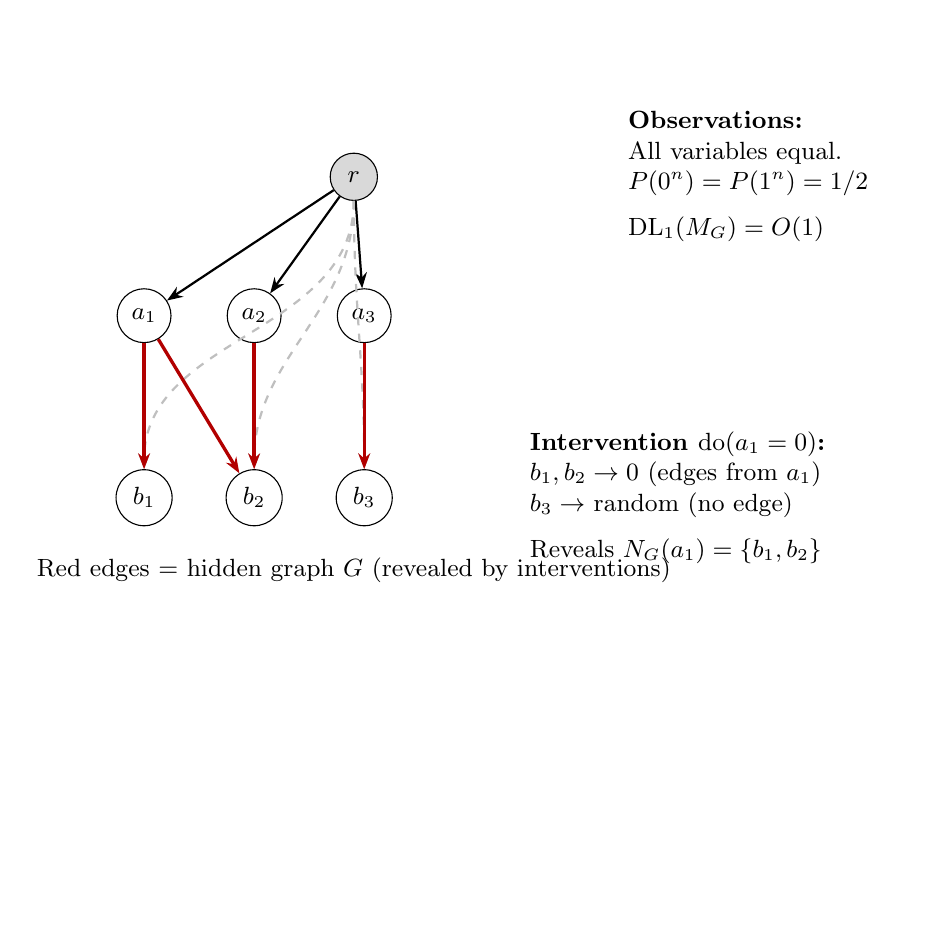
\begin{tikzpicture}[
        node distance=0.9cm,
        every node/.style={circle, draw, minimum size=0.6cm, font=\small},
        arr/.style={-{Stealth[length=2mm]}, thick}
    ]
    % Root
    \node (R) [fill=gray!30] {$r$};
    
    % Layer A
    \node (A1) [below left=1.3cm and 2.2cm of R] {$a_1$};
    \node (A2) [right=0.7cm of A1] {$a_2$};
    \node (A3) [right=0.7cm of A2] {$a_3$};
    
    % Layer B
    \node (B1) [below=1.6cm of A1] {$b_1$};
    \node (B2) [below=1.6cm of A2] {$b_2$};
    \node (B3) [below=1.6cm of A3] {$b_3$};
    
    % Root to A edges (solid)
    \draw[arr] (R) -- (A1);
    \draw[arr] (R) -- (A2);
    \draw[arr] (R) -- (A3);
    
    % Root to B edges (dashed, implicit)
    \draw[arr, gray!50, dashed] (R) to[out=-90, in=90] (B1);
    \draw[arr, gray!50, dashed] (R) to[out=-90, in=90] (B2);
    \draw[arr, gray!50, dashed] (R) to[out=-90, in=90] (B3);
    
    % Bipartite edges G (red, the hidden structure)
    \draw[arr, red!70!black, very thick] (A1) -- (B1);
    \draw[arr, red!70!black, very thick] (A1) -- (B2);
    \draw[arr, red!70!black, very thick] (A2) -- (B2);
    \draw[arr, red!70!black, very thick] (A3) -- (B3);
    
    % Annotations
    \node[draw=none, right=2.8cm of R, align=left, font=\small] {
        \textbf{Observations:}\\
        All variables equal.\\
        $P(0^n) = P(1^n) = 1/2$\\[0.2cm]
        $\DL_1(M_G) = O(1)$
    };
    
    \node[draw=none, right=2.8cm of B2, align=left, font=\small] {
        \textbf{Intervention $\doop(a_1 = 0)$:}\\
        $b_1, b_2 \to 0$ (edges from $a_1$)\\
        $b_3 \to$ random (no edge)\\[0.2cm]
        Reveals $N_G(a_1) = \{b_1, b_2\}$
    };
    
    % Legend
    \node[draw=none] at (0, -5) {\small Red edges = hidden graph $G$ (revealed by interventions)};
    
    \end{tikzpicture}
    \caption{\textbf{The Bipartite-Graph Construction.} The root $r$ feeds into layer $A$ (copy), and layer $A$ feeds into layer $B$ via AND gates controlled by graph $G$ (red edges). Observationally, all $2^{m^2}$ choices of $G$ produce the same distribution. Interventions on layer $A$ reveal which layer-$B$ nodes are neighbors.}
    \label{fig:bipartite-construction}
\end{figure}

\begin{figure}[t]
    \centering
    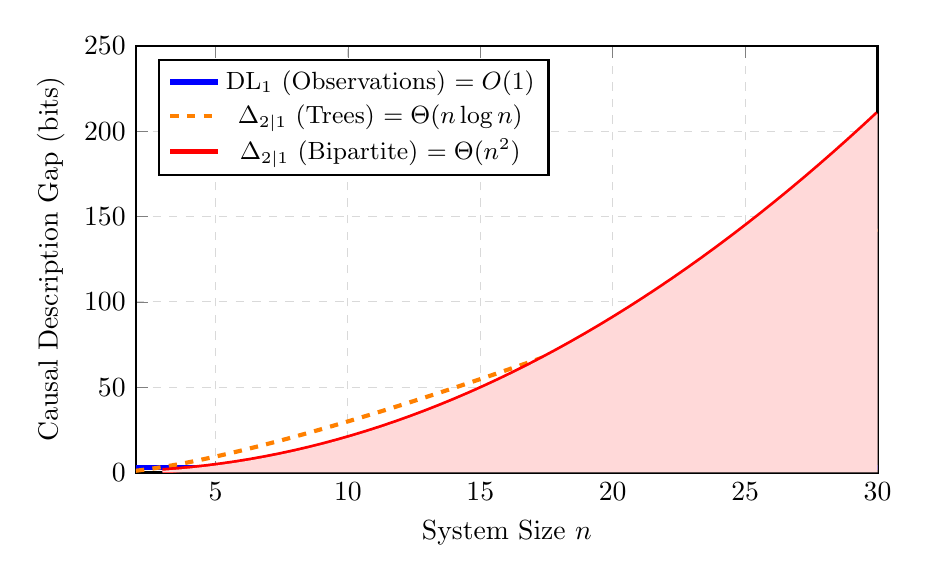
\begin{tikzpicture}
        \begin{axis}[
            width=11cm, height=7cm,
            xlabel={System Size $n$},
            ylabel={Causal Description Gap (bits)},
            xmin=2, xmax=30, ymin=0, ymax=250,
            legend pos=north west,
            legend style={font=\small},
            grid=major, grid style={dashed, gray!30}, thick
        ]
        \addplot[color=blue, line width=2pt, domain=2:30, samples=50] {3};
        \addlegendentry{$\DL_1$ (Observations) $= O(1)$}
        \addplot[color=orange, line width=1.5pt, dashed, domain=2:30, samples=50] {(x-1)*ln(x)/ln(2)};
        \addlegendentry{$\Delta_{2|1}$ (Trees) $= \Theta(n \log n)$}
        \addplot[color=red, line width=2pt, domain=3:30, samples=50] {((x-1)/2)^2};
        \addlegendentry{$\Delta_{2|1}$ (Bipartite) $= \Theta(n^2)$}
        \addplot[fill=red!15, draw=none, domain=3:30, samples=50] {((x-1)/2)^2} \closedcycle;
        \end{axis}
    \end{tikzpicture}
    \caption{\textbf{The Causal Description Gap grows quadratically.} Observational description length (blue) is constant. The tree construction (orange) achieves $\Theta(n \log n)$. The bipartite construction (red) achieves $\Theta(n^2)$, a quadratic gap between knowing ``what happens'' and knowing ``why.''}
    \label{fig:gap-comparison}
\end{figure}

\begin{proof}[Proof of Lemma~\ref{lem:bipartite-obs}]
We analyze the two cases for the root's value.

\textbf{Case $U_r = 0$:} Then $X_r = 0$. Since each $X_{a_i} = X_r$, we have $X_{a_i} = 0$ for all $i$. For each $b_j$, the equation is:
\[
X_{b_j} = X_r \wedge \bigwedge_{a_i : (a_i, b_j) \in G} X_{a_i} = 0 \wedge (\cdots) = 0.
\]
Thus all variables are $0$.

\textbf{Case $U_r = 1$:} Then $X_r = 1$ and $X_{a_i} = 1$ for all $i$. For each $b_j$:
\[
X_{b_j} = X_r \wedge \bigwedge_{a_i : (a_i, b_j) \in G} X_{a_i} = 1 \wedge 1 \wedge \cdots \wedge 1 = 1.
\]
(If $b_j$ has no neighbors, the empty AND is $1$, so $X_{b_j} = 1 \wedge 1 = 1$.)

Thus all variables are $1$.

Since $U_r \sim \mathrm{Bernoulli}(1/2)$, the outcome is $0^n$ or $1^n$ each with probability $1/2$. This is $P^\star$, independent of $G$.
\end{proof}

\begin{proof}[Proof of Lemma~\ref{lem:bipartite-intervention}]
Under $\doop(X_{a_i} = 0)$, the equation for $X_{a_i}$ becomes $X_{a_i} := 0$. The root $X_r = U_r$ remains random, and all other layer-$A$ nodes satisfy $X_{a_k} = X_r$ for $k \neq i$.

\textbf{Case $(a_i, b_j) \in G$:} The equation for $X_{b_j}$ includes $X_{a_i}$ as an AND input:
\[
X_{b_j} = X_r \wedge X_{a_i} \wedge \bigwedge_{a_k \neq a_i : (a_k, b_j) \in G} X_{a_k}.
\]
Since $X_{a_i} = 0$, the AND evaluates to $0$ regardless of other inputs. Thus $X_{b_j} = 0$ deterministically, so $P(X_{b_j} = 0) = 1$.

\textbf{Case $(a_i, b_j) \notin G$:} The equation for $X_{b_j}$ does not include $X_{a_i}$:
\[
X_{b_j} = X_r \wedge \bigwedge_{a_k : (a_k, b_j) \in G} X_{a_k}.
\]
All terms in this AND equal $X_r$ (since $X_{a_k} = X_r$ for $k \neq i$). If there are $d$ such terms:
\[
X_{b_j} = X_r \wedge X_r \wedge \cdots \wedge X_r = X_r.
\]
(If $b_j$ has no neighbors other than possibly $a_i$, and $(a_i, b_j) \notin G$, then the AND is either empty (giving $X_{b_j} = X_r$) or involves only other $a_k$ that equal $X_r$.)

Thus $X_{b_j} = X_r \sim \mathrm{Bernoulli}(1/2)$, so $P(X_{b_j} = 0) = 1/2$.
\end{proof}

\begin{proof}[Proof of Lemma~\ref{lem:bipartite-injective}]
By Lemma~\ref{lem:bipartite-intervention}, from $\Int_1(M_G)$ we can extract:
\[
N_G(a_i) = \{b_j \in B : P_{M_G}^{\doop(X_{a_i} = 0)}(X_{b_j} = 0) = 1\}
\]
for each $a_i \in A$. The neighborhoods $\{N_G(a_i)\}_{i=1}^m$ determine all edges of $G$:
\[
(a_i, b_j) \in G \iff b_j \in N_G(a_i).
\]
Thus $\Int_1(M_G)$ determines $G$ uniquely.
\end{proof}

\begin{proof}[Proof of Theorem~\ref{thm:quadratic-separation}]
\textbf{Lower bound:} There are $2^{m^2}$ bipartite graphs $G \subseteq A \times B$ (each of the $m^2$ potential edges is present or absent). By Lemma~\ref{lem:bipartite-injective}, there are $2^{m^2}$ distinct interventional families. By Lemma~\ref{lem:bipartite-obs}, all share $\Obs(M_G) = P^\star$ with $\DL_1 = O(1)$.

By the counting bound: among $2^{m^2}$ distinct strings, at least one has Kolmogorov complexity $\geq m^2 - O(1)$. By Lemma~\ref{lem:conditioning-simple}, $\Delta_{2|1}(M_G) = \DL_2(M_G) \pm O(\log n)$.

The high-probability statement follows from the stronger counting bound: all but a $2^{-c}$ fraction have complexity $\geq m^2 - c - O(1)$.

\textbf{Upper bound:} The graph $G$ can be encoded as an $m \times m$ binary adjacency matrix, requiring $m^2$ bits. Given $G$ and $n$, a constant-length program simulates $M_G$ and outputs $\Int_1(M_G)$. Thus $K(\Int_1(M_G) \mid n) \leq m^2 + O(1)$.
\end{proof}

\begin{proof}[Proof of Theorem~\ref{thm:degree-upper}]
An SCM in $\calM_{n,d}(\Gamma,\Pi)$ can be encoded by listing:
\begin{enumerate}
    \item a topological ordering of the $n$ variables, using $O(n \log n)$ bits;
    \item for each variable, its parent set, chosen from at most $\sum_{k=0}^{d} \binom{n-1}{k}$ possibilities;
    \item for each variable, a gate from the fixed library $\Gamma$ and a noise distribution from the fixed library $\Pi$, using $O(1)$ bits per variable.
\end{enumerate}
The entire SCM thus has a description of length
\[
    O(n \log n) + n \log_2\!\Bigl(\sum_{k=0}^{d} \binom{n-1}{k}\Bigr) + O_{\Gamma,\Pi}(n).
\]
Given this description and $n$, a fixed program can compute all single-node interventional distributions and output $\Int_1(M)$. Hence the same expression upper-bounds $K(\Int_1(M) \mid n) = \DL_2(M)$.

Finally,
\[
    \sum_{k=0}^{d} \binom{n-1}{k} \;\leq\; (d+1) \left(\frac{e(n-1)}{d}\right)^d
\]
for $1 \leq d \leq n-1$, yielding the stated asymptotic form. Since $\Delta_{2|1}(M) \leq \DL_2(M) + O(1)$, the same upper bound applies to the gap.
\end{proof}

\begin{proof}[Proof of Theorem~\ref{thm:approx-quadratic}]
\textbf{Upper bound.} An exact $m^2$-bit encoding of $G$ as an $m \times m$ binary adjacency matrix lets a fixed program output $\Int_1(M_G)$ exactly, hence also $\varepsilon$-approximately for any $\varepsilon \geq 0$. So $K_\varepsilon(\Int_1(M_G) \mid \Obs(M_G), n) \leq m^2 + O(1)$.

\textbf{Lower bound.} Let $G \neq G'$ be two distinct bipartite graphs. They differ on some edge $(a_i, b_j)$; WLOG $(a_i, b_j) \in G$ and $(a_i, b_j) \notin G'$. By Lemma~\ref{lem:bipartite-intervention},
\[
    P_{M_G}^{\doop(X_{a_i} = 0)}(X_{b_j} = 0) = 1, \qquad P_{M_{G'}}^{\doop(X_{a_i} = 0)}(X_{b_j} = 0) = 1/2.
\]
Total variation distance does not increase under marginalization, so the full interventional distributions satisfy
\[
    \mathrm{TV}\!\bigl( P_{M_G}^{\doop(X_{a_i} = 0)},\; P_{M_{G'}}^{\doop(X_{a_i} = 0)} \bigr) \;\geq\; \tfrac{1}{2}.
\]
Hence $d_{\Int}(\Int_1(M_G), \Int_1(M_{G'})) \geq 1/2$. For $\varepsilon < 1/4$, the open $\varepsilon$-balls around the $2^{m^2}$ answer objects are pairwise disjoint, so any $\varepsilon$-accurate description must still distinguish among $2^{m^2}$ possibilities. Applying the conditional counting bound (Lemma~\ref{lem:counting}, part~2) with the common observation $P^\star$ as side information yields the existence and high-probability lower bounds.
\end{proof}

\section{Modular-XOR Construction: Full Proofs}
\label{app:xor-proofs}

This appendix supports Section~\ref{sec:counterfactual}. We prove, in order, Lemmas~\ref{lem:xor-obs} (observational equivalence), \ref{lem:xor-int} (single-node interventional equivalence), \ref{lem:xor-cf} (counterfactual encoding is injective in $s$), \ref{lem:xor-all-int} (indistinguishability under \emph{all} atomic interventions), and Theorem~\ref{thm:cf-separation} (the $\Theta(n)$ counterfactual gap conditional on $\Int_{\mathrm{all}}$).

\begin{proof}[Proof of Lemma~\ref{lem:xor-obs}]
We show each module $(X_t, Y_t)$ is uniformly distributed on $\{0,1\}^2$.

\textbf{Case $s_t = 0$:} $X_t = U_{X_t}$ and $Y_t = U_{Y_t}$ are independent $\mathrm{Bernoulli}(1/2)$ variables.

\textbf{Case $s_t = 1$:} $X_t = U_{X_t} \sim \mathrm{Bernoulli}(1/2)$. For $Y_t = X_t \oplus U_{Y_t}$: for any fixed $x \in \{0,1\}$,
\[
\Prob(Y_t = y \mid X_t = x) = \Prob(U_{Y_t} = x \oplus y) = 1/2.
\]
Thus $Y_t$ is uniform and independent of $X_t$. (Formally: $\Prob(X_t = x, Y_t = y) = \Prob(X_t = x) \Prob(Y_t = y) = 1/4$.)

Since modules are independent and each is uniform on $\{0,1\}^2$, the full distribution is uniform on $\{0,1\}^{2m}$.
\end{proof}

\begin{proof}[Proof of Lemma~\ref{lem:xor-int}]
Consider any single-variable intervention $\doop(X_t = x)$ or $\doop(Y_t = y)$.

\textbf{Intervention $\doop(X_t = x)$:} The equation $X_t := x$ replaces whatever $X_t$ was. In module $t$:
\begin{itemize}
    \item If $s_t = 0$: $Y_t = U_{Y_t}$, uniform.
    \item If $s_t = 1$: $Y_t = x \oplus U_{Y_t}$, also uniform (since $U_{Y_t}$ is uniform).
\end{itemize}
Either way, $Y_t$ is uniform and independent of the intervention value. Other modules are unaffected.

\textbf{Intervention $\doop(Y_t = y)$:} The equation $Y_t := y$ replaces whatever $Y_t$ was. In both cases ($s_t = 0$ or $1$), $X_t = U_{X_t}$ remains uniform. Other modules unaffected.

Since all single-variable interventional distributions are the same across all $s$, the entire family $\Int_1(M_s)$ is independent of $s$.
\end{proof}

\begin{proof}[Proof of Lemma~\ref{lem:xor-cf}]
For each module $t$, consider the counterfactual query: ``What is $\Prob(Y_t^{(X_t \leftarrow 0)} = Y_t^{(X_t \leftarrow 1)})$?''

Let $Y_t^{(X_t \leftarrow b)}$ denote the value of $Y_t$ when we intervene with $\doop(X_t = b)$, evaluated on the same noise $U_{Y_t}$.

\textbf{Case $s_t = 0$:} $Y_t^{(X_t \leftarrow 0)} = U_{Y_t}$ and $Y_t^{(X_t \leftarrow 1)} = U_{Y_t}$. These are identical, so $\Prob(Y_t^{(X_t \leftarrow 0)} = Y_t^{(X_t \leftarrow 1)}) = 1$.

\textbf{Case $s_t = 1$:} $Y_t^{(X_t \leftarrow 0)} = 0 \oplus U_{Y_t} = U_{Y_t}$ and $Y_t^{(X_t \leftarrow 1)} = 1 \oplus U_{Y_t} = 1 - U_{Y_t}$. These are always different, so $\Prob(Y_t^{(X_t \leftarrow 0)} = Y_t^{(X_t \leftarrow 1)}) = 0$.

Thus the counterfactual query for module $t$ outputs $1$ if $s_t = 0$ and $0$ if $s_t = 1$. The $m$ queries together determine $s$.

Since $\CF_1(M_s)$ contains $P(X, X^{(t \leftarrow 0)}, X^{(t \leftarrow 1)})$ for all $t$, which includes the joint distribution of $Y_t^{(X_t \leftarrow 0)}$ and $Y_t^{(X_t \leftarrow 1)}$, it determines $s$.
\end{proof}

\begin{proof}[Proof of Lemma~\ref{lem:xor-all-int}]
It suffices to consider a single module $(X_t, Y_t)$, since modules are independent and interventions factor across modules. Fix an arbitrary intervention on any subset of $\{X_t, Y_t\}$.

If $Y_t$ is intervened on, then $Y_t$ is fixed by the intervention. The remaining variable $X_t$, if not intervened on, equals $U_{X_t}$ and is uniform in both the no-effect and XOR mechanisms.

If $Y_t$ is not intervened on but $X_t$ is set to $x$, then
\[
    Y_t = \begin{cases} U_{Y_t}, & s_t = 0,\\ x \oplus U_{Y_t}, & s_t = 1. \end{cases}
\]
In either case $Y_t$ is uniform Bernoulli and independent of all other modules.

Finally, if neither variable is intervened on, then for $s_t = 0$ we have $(X_t, Y_t) = (U_{X_t}, U_{Y_t})$, uniform on $\{0,1\}^2$; for $s_t = 1$ we have $(X_t, Y_t) = (U_{X_t}, U_{X_t} \oplus U_{Y_t})$, also uniform on $\{0,1\}^2$.

Thus every possible intervention produces the same distribution regardless of $s_t$. Taking the product over independent modules proves the claim.
\end{proof}

\begin{proof}[Proof of Theorem~\ref{thm:cf-separation}]
\textbf{Part 1.} By Lemma~\ref{lem:xor-all-int}, $\Int_{\mathrm{all}}(M_s)$ is identical for all $s$. Its description is constant: every intervention fixes the intervened variables and leaves each non-intervened module uniformly distributed in the manner described in the proof of Lemma~\ref{lem:xor-all-int}.

\textbf{Part 2 (Upper bound).} Given $s$ ($m$ bits) and $n$, a constant-length program simulates $M_s$ and outputs $\CF_1(M_s)$. Thus $K(\CF_1(M_s) \mid n) \leq m + O(1)$.

\textbf{Part 3 (Lower bound).} By Lemma~\ref{lem:xor-cf}, the map $s \mapsto \CF_1(M_s)$ is injective. Hence there are $2^m$ distinct counterfactual answer objects consistent with the same full hard-do interventional oracle. The conditional counting bound (Lemma~\ref{lem:counting}, part~2), applied with $w = (\Int_{\mathrm{all}}(M_s), n)$, yields the high-probability claim, since $\Int_{\mathrm{all}}(M_s)$ is constant across $s$ and contributes only $O(1)$ to the conditioning.
\end{proof}

\section{Learning-Theoretic Consequences}
\label{app:learning}

This appendix supports the brief discussion of \S\ref{sec:learning-main} of the main paper. We give two no-free-lunch results for observational learners drawn from the bipartite family $\calM_{\mathrm{bip}}^n$ (Definition~\ref{def:bipartite-scm}): one bounds the joint-recovery success rate, the other a per-query absolute error.

\begin{corollary}[No-free-lunch for observational learners]
\label{cor:no-free-lunch}
Let $G \sim \mathrm{Unif}(2^{A \times B})$ in the bipartite family $\calM_{\mathrm{bip}}^n$. Any learner $\calA$ that receives an i.i.d.\ sample of any size from $\Obs(M_G)$ and outputs a prediction $\widehat{\Int}_1$ satisfies
\[
\Prob[\widehat{\Int}_1 = \Int_1(M_G)] \;\leq\; 2^{-m^2}.
\]
\end{corollary}

\begin{proof}
All $M_G$ share the observational distribution $P^\star$, so any sample from $P^\star$ is statistically independent of $G$. The learner's output, a function of the sample, is therefore independent of $G$. With $2^{m^2}$ equiprobable targets $\{\Int_1(M_G)\}$ (the map $G \mapsto \Int_1(M_G)$ is injective by Lemma~\ref{lem:bipartite-injective}) and output independent of the true target, the success probability is at most $2^{-m^2}$.
\end{proof}

\begin{corollary}[Per-query prediction error]
\label{cor:per-query-error}
Let $G \sim \mathrm{Unif}(2^{A \times B})$ in the bipartite family $\calM_{\mathrm{bip}}^n$. Let $\hat{p}$ be any predictor (possibly depending on an i.i.d.\ sample of any size from $\Obs(M_G)$). For an independent uniformly random pair $(i,j) \in [m] \times [m]$, let $p_{i,j}(G) := P_{M_G}^{\doop(X_{a_i} = 0)}(X_{b_j} = 0)$. Then
\[
\E\bigl[|\hat{p}_{i,j} - p_{i,j}(G)|\bigr] \;\geq\; \tfrac{1}{4}.
\]
\end{corollary}

\begin{proof}
By Lemma~\ref{lem:bipartite-intervention}, $p_{i,j}(G) \in \{1/2, 1\}$ depending on whether $(a_i, b_j) \in G$. For $G \sim \mathrm{Unif}(2^{A \times B})$ the edge indicator is Bernoulli$(1/2)$, so $p_{i,j}(G)$ equals $1$ and $1/2$ each with probability $1/2$. The observational sample is independent of $G$, hence so is the predictor output $\hat{p}_{i,j}$. Condition on $\hat{p}_{i,j} = a$:
\[
\E\bigl[|\hat{p}_{i,j} - p_{i,j}(G)| \,\big|\, \hat{p}_{i,j} = a\bigr] \;=\; \tfrac{1}{2} |a - 1| + \tfrac{1}{2} |a - \tfrac{1}{2}| \;\geq\; \tfrac{1}{4},
\]
where the last step uses the triangle inequality $|a-1| + |a-\tfrac{1}{2}| \geq |1 - \tfrac{1}{2}| = \tfrac{1}{2}$. Averaging over $a$ proves the claim.
\end{proof}

This is not a computational limitation; it is information-theoretic. No algorithm, however powerful, can reliably predict interventional outcomes from observations when the underlying mechanism is drawn from our family.

\begin{remark}[Shannon Mutual Information is Zero]
\label{rem:mutual-info}
In the bipartite family $\calM_{\mathrm{bip}}^n$, a dataset $D \sim (P^\star)^N$ of $N$ i.i.d.\ observational samples is independent of the hidden graph $G$, since all mechanisms share the same observational distribution. Therefore $I(G; D) = 0$ in the Shannon sense for every sample size $N$. The lower bounds in Corollary~\ref{cor:no-free-lunch} and Corollary~\ref{cor:per-query-error} follow from this information-theoretic independence and do not rely on uncomputability of Kolmogorov complexity.
\end{remark}

%==============================================================================
% NeurIPS checklist intentionally omitted from arXiv version.

\end{document}
